In general, analyses at the \LHC fall under one of two broad categories: they are either measurements (which, to this day, have shown to agree with the Standard Model), or direct searches for beyond the Standard Model physics. Although direct searches are precise and sensitive to the targeted new physics signals, they tend to very model dependent and cover only a small subset of all possible theories and parameter space. Furthermore, an \LHC search can take from months to years from inception to publication. There is simply not enough person- or computing-power to conduct a direct search for every BSM model on the market. A solution to this well-known problem lies in the former category of \LHC results: the measurements. The idea is that the addition of a new particle or new interaction would affect observables that have already been precisely measured. Therefore a good handful of models may already be excluded, given that so far, no excesses have been observed. 

This idea is a bottom-up, data-driven approach at probing BSM models. In the particle physics community, the reuse of data after its publication is called re-interpretation. Re-interpretation allows a much larger breadth of BSM models to be tested outside of the experimental collaborations by theorists and experimentalists alike. Given how time consuming it is to do physics analyses, it is in the interest of the particle physics community to maximize the scientific impact of published data by ensuring reinterpretability. Although it is not a tool for discovery, reinterpretation studies are often useful in helping experiments identify plausible BSM scenarios that direct searches should target. Since they make use of existing results, they do not require any reprocessing of the data, event selection, or background and systematics estimates. It is considered good practice for analysis teams to publish, along with their measurement, material for reinterpretation. The latest report from the \LHC reinterpretation forum can be found in Reference~\cite{reinterpretation_forum}, which details the recommendations that analysis teams can take to ensure reinterpretability.

In this Chapter, an overview of the philosophy and workflow behind the \contur reinterpretation package is given. Two reinterpretation studies are presented where existing \LHC measurements are used to set limits in previously unexplored regions of BSM model space. The \ATLAS four-lepton measurement of Chapter~\ref{chap:fourlepton} plays a particularly important role in both, and is studied in detail. First, section~\ref{sec:reinterpretsoftware} introduces \contur, from which the results are derived for the rest of this Chapter. Section~\ref{sec:VLQ} is adapted from Reference~\cite{VLQ_contur}, where limits are set by \LHC measurements on a BSM particles vector-like quarks. Finally, section~\ref{sec:BL} shows the results of a brief study on a model with a gauged $B-L$ symmetry.

\section{\contur and related software tools}
\label{sec:reinterpretsoftware}
This section provides a brief summary of the \contur method, adapted from key paragraphs of the manual. For more comprehensive explanations, please refer to the relevant sections of the manual.

The backbone of the \contur method lies in the fact that many differential cross-sections are precisely measured and well understood, and that any modifications to the SM Lagrangian would inevitably introduce changes to these cross-sections. If the change induced by adding in a new particle or a new field is beyond the well data's uncertainties, then (quoting the manual) "we'd already have seen it". In other words, if one can predict the changes to the hundreds of \LHC measured distributions that a BSM model would make, then one can already determine what regions of the model's parameter space are already excluded. This is the philosophy upon which \contur was built. 

A couple of ingredients are necessary for running \contur. First, the BSM model must be interfaced to a Monte Carlo event generator in order to simulate events. Facilitating this procedure is the \FeynRules~\cite{}. At its core, \FeynRules is a mathematica package used to develop BSM models. Upon the input of a Lagragian, it derives the Feynman rules. An important feature is the export to the Universal FeynRules Object~\cite{ufo} (UFO) format, compatible with a range of event generators. UFO files hold the basic information about new particles and parameters which are directly used to generate events for new physics signals. The MC event generator used for studies in this thesis is \herwig~\cite{herwig7}, the default MC event generator used by \contur. It is important to note here another pillar in the \contur philosophy: to use inclusive event generation wherever possible. The advantage of doing so is the coverage of all allowed final states which would be affected if that BSM model were to exist. \todo{Reword this last sentence!!!}Generating events inclusively rather than exclusively allows \contur to paint a comprehensive picture of the exclusion across all manner of final states instead of focusing on the most spectacular signatures of a new model~\cite{contur-manual}. 

Second, a platform to compare the simulated BSM events to the plethora of LHC measurements is needed. This job is done by \rivet~\cite{rivet}, a general-purpose tool used to reproduce analysis procedures on simulated events. It hosts a wealth of measurements from various high energy physics experiments. Each measurement is written into a \rivet routine which preserves the workflow of the analysis. Included are crucial information such as the fiducial region selection cuts and observable binnings. With this information, \rivet is able to transform the output from Monte Carlo event generators into histograms of cross-sections in the scope of the measurement. In general, it is considered good practice for \LHC measurements to publish their data on \HEPData~\cite{HEPData} and to provide the analysis code as a \rivet routine. \rivet's growing library of available analyses and it's ability to make fast and easy to comparisons between raw generator output and particle-level data is the foundation upon which \contur is built. 

The \contur workflow is summarized in Figure~\ref{fig:conturworkflow} in four steps, taken from Reference~\cite{conturmanual}. Each step is written in bold, with the tool used to achieve it in smaller font. First in the workflow is to call upon an event generator (e.g. \herwig) to simulate new physics events for a specified BSM model. The free paramters of the BSM model should be defined manually by the user. \herwig is interfaced to \rivet directly so the events are directly piped into the observables' histograms. The \rivet output corresponds to the excess BSM contribution in any of the measured distributions made at the \LHC which would be present should the model hold true. The next step is to evaluate the likelihood for the BSM model given the size of the measurement uncertainty. The heap of measurements are grouped into orthogonal pools based on their final state signature, and \contur uses the best constraint from each pool to form a global exclusion measure for a given model at a given set of parameter values~\cite{contur-manual}. This is \contur's main functionality, and takes around one hour to complete for a single model parameter point. The same process is repeated for many points in a two-dimensional grid of the BSM model's parameter values. With the help of a computing farm with multiple nodes, this can be done in less than one workday. Finally, \contur's plotting functions allow the user to visualize the likelihood evaluation of their scanned parameter space. Like so, \contur is able to tell the user whether wide regions of the BSM model's parameter is already exluded by \LHC previous measurements. An in depth description of each step can be found in Reference~\cite{conturmanual}. 
\begin{figure}
  \begin{center}
    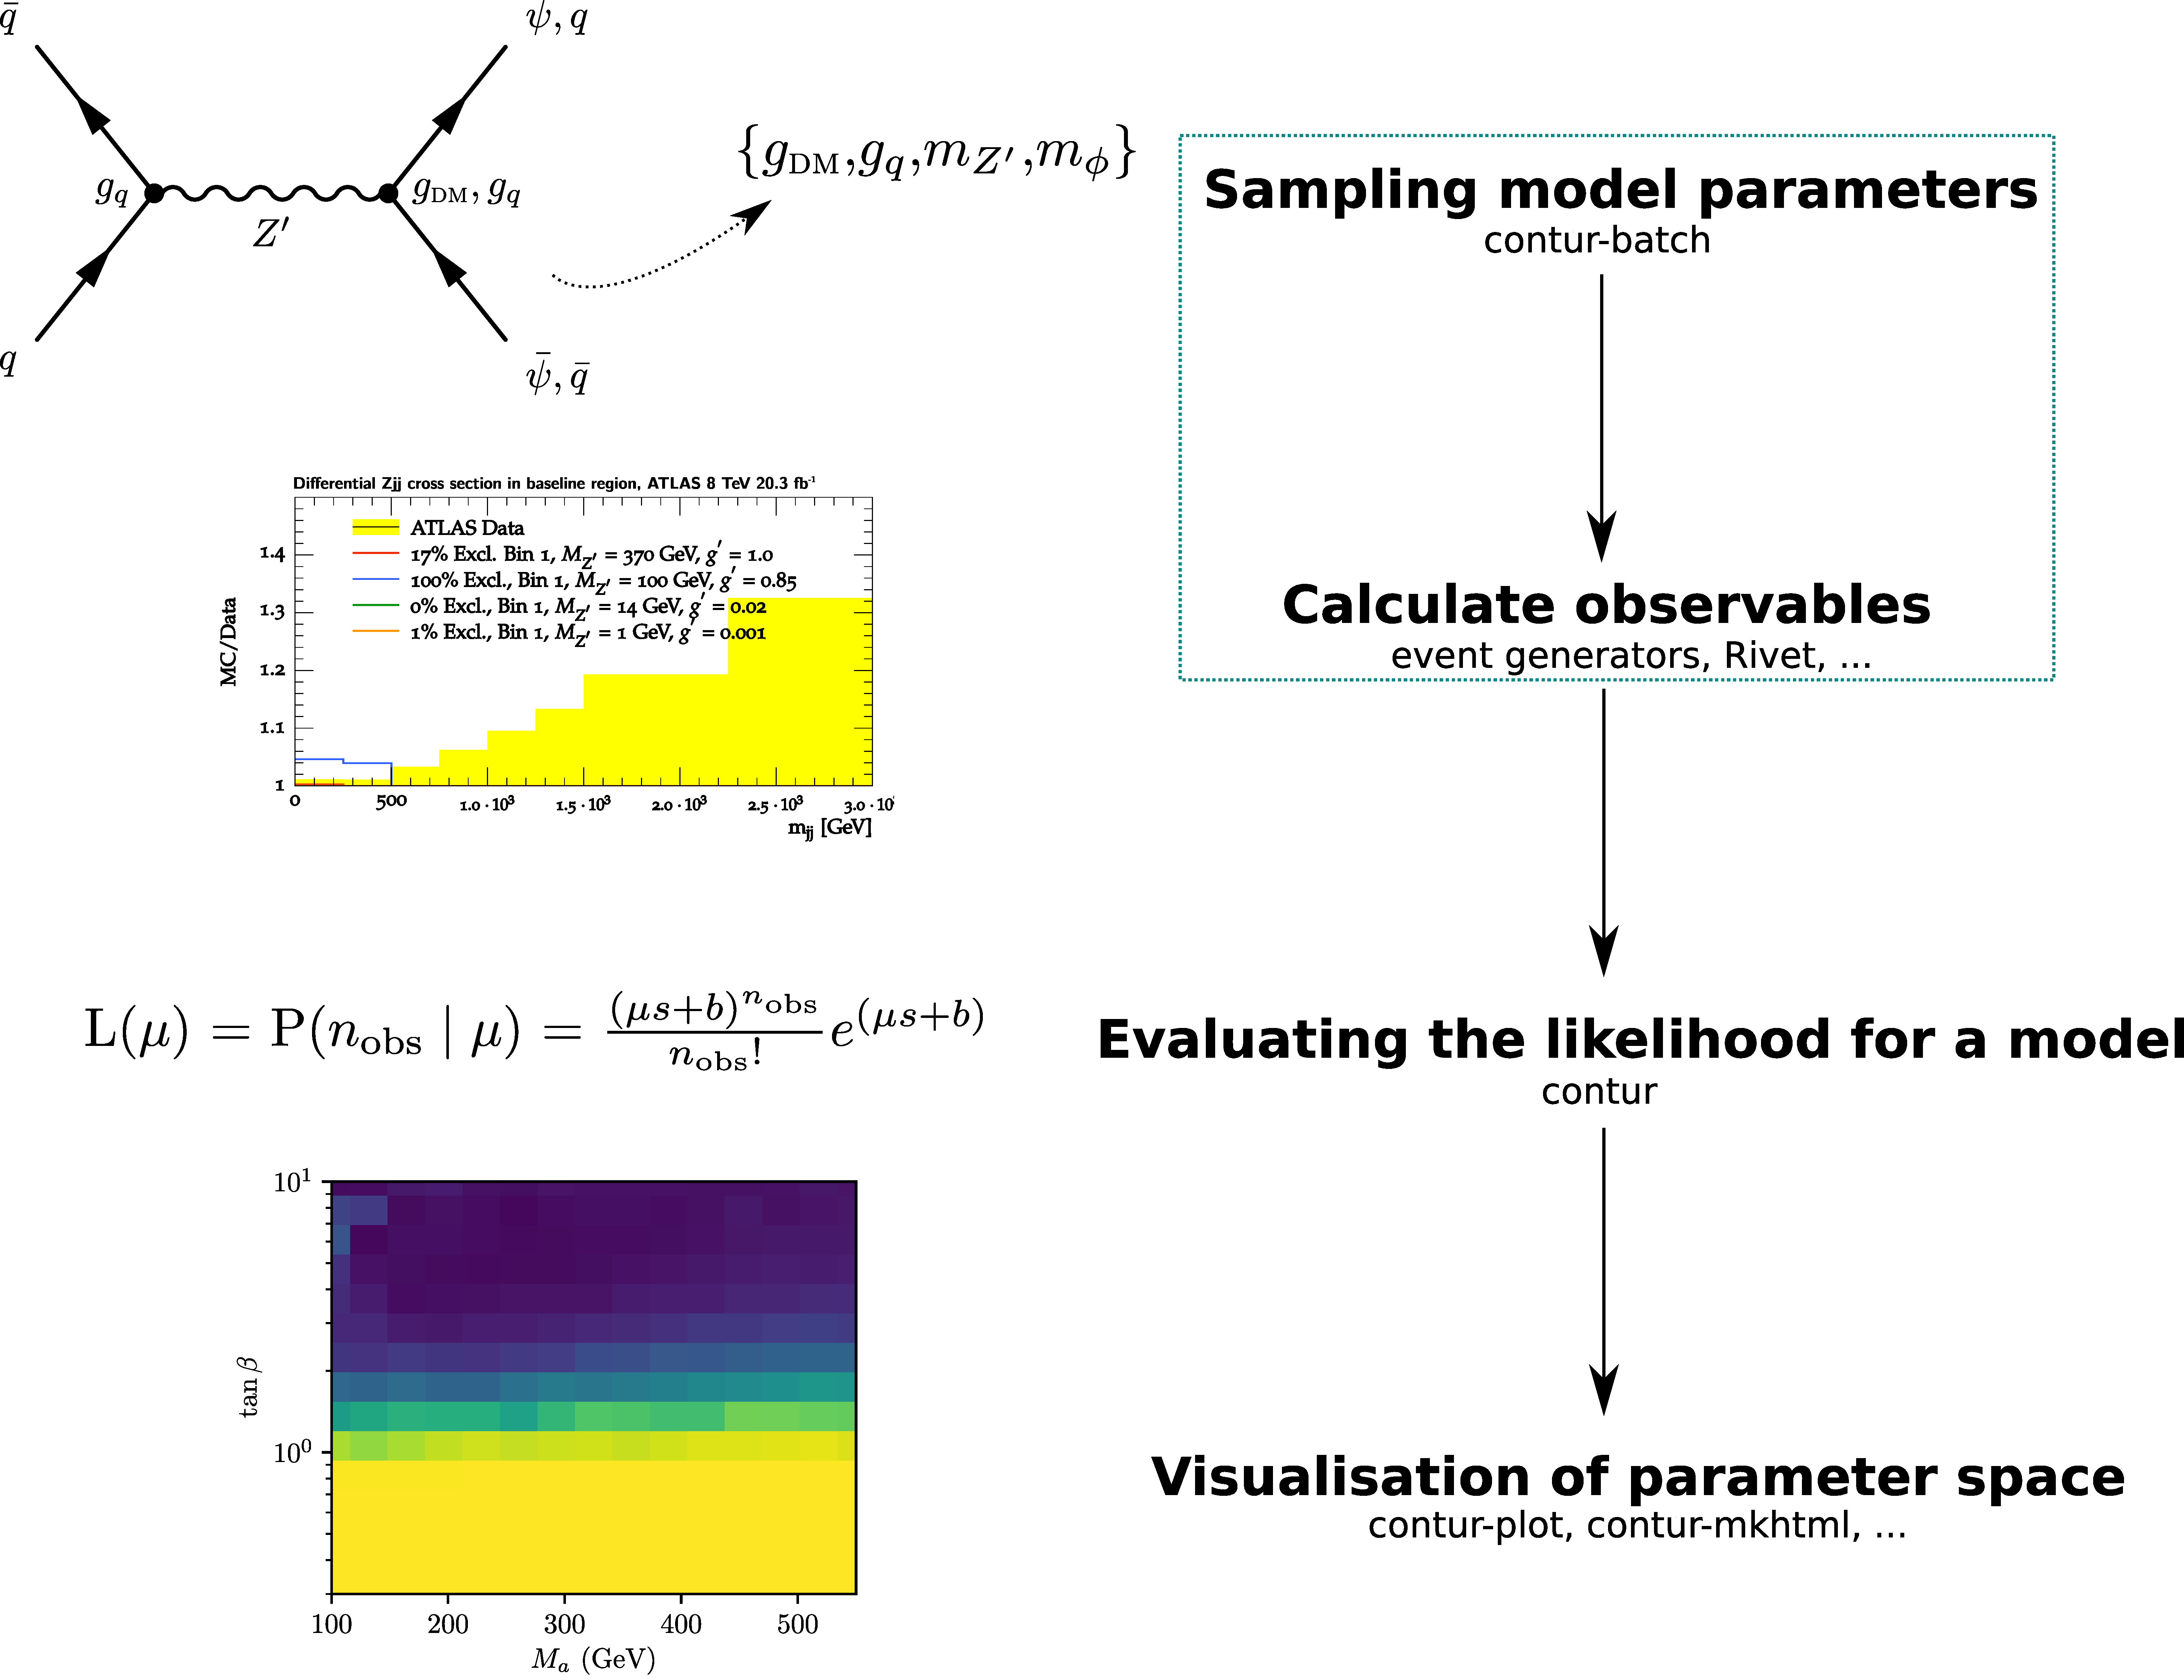
\includegraphics[width=1.0\textwidth]{Figures/contur/workflow.pdf}
    \caption{An simplified schematic of the \contur workflow. The dotted box denotes the portion of the workflow that makes extensive use of external packages, affording multiple options, such as the choice of MC event generator. The next stage is the taking of physics observables as inputs to a statistical analysis (i.e. evaluating the likelihood for the model). Finally the last stage involves using tools to visualize the output of the likelihood analysis. Figure taken from Reference~\cite{conturmanual}}.
    \label{fig:conturworkflow}
  \end{center}
\end{figure}